\begin{frame}[fragile,t]
\frametitle{\hfill}
\MyHeading{\ED Project}
% \vspace{\mytopbit}
\vspace{0.1in}
\begin{center}
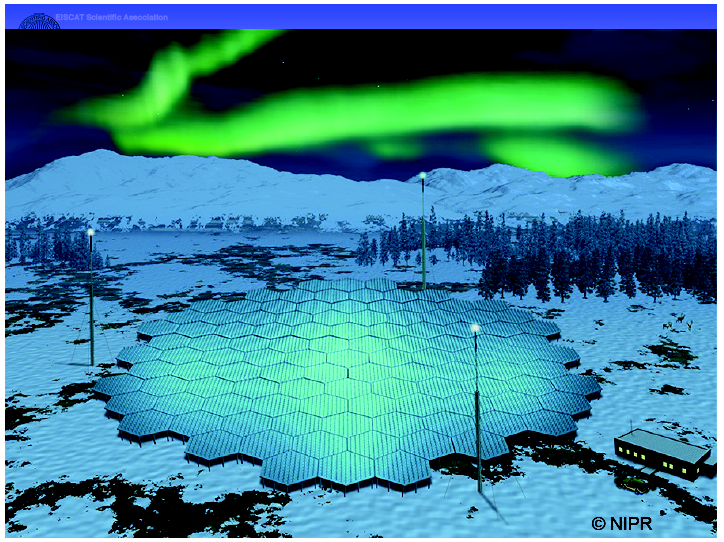
\includegraphics[height=2.7in]{eiscat_3d_array.png}
% \end{center}
% \vspace{-0.60in}
\vfill
% \note{\bitm 
    {\colblack 109 Arrays of 91 antennas. VHF 233 MHz. Solid state amplifiers.\\Up to 100 simultaneous beams. 60$^\circ$ zenith angle}
    {\colblack \small \url{https://www.eiscat.se/about/eiscat3d7/}}
% \vfill
\end{center}
%       \item dimensions... 6m/80m dia.
%        \item TX 10 MW, high/low power modes, 
%        \item 60 degrees zenith angle, 
%        \item micro-second direction in point/look
%        \item white rabbit on-site
%        \item GPS between sites
%        \item explain time/volume integration for 3d operations
%       \eitm}
\end{frame}

\begin{frame}[fragile,t]
\frametitle{\hfill}
\MyHeading{\ED Project}
% \vspace{\mytopbit}
\vspace{0.1in}
\begin{center}
% 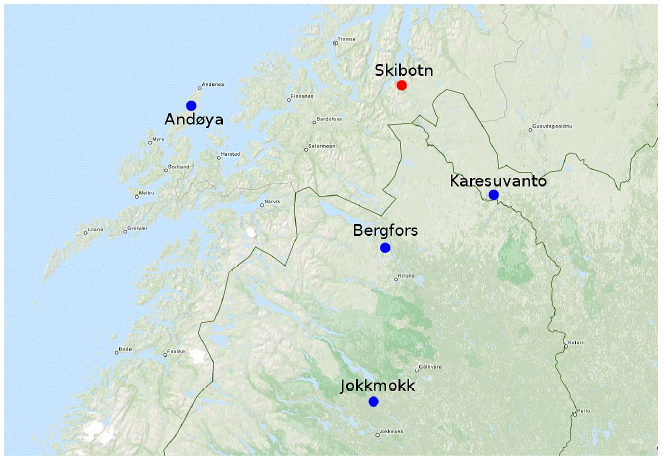
\includegraphics[height=2.7in]{eiscat-sites.png}
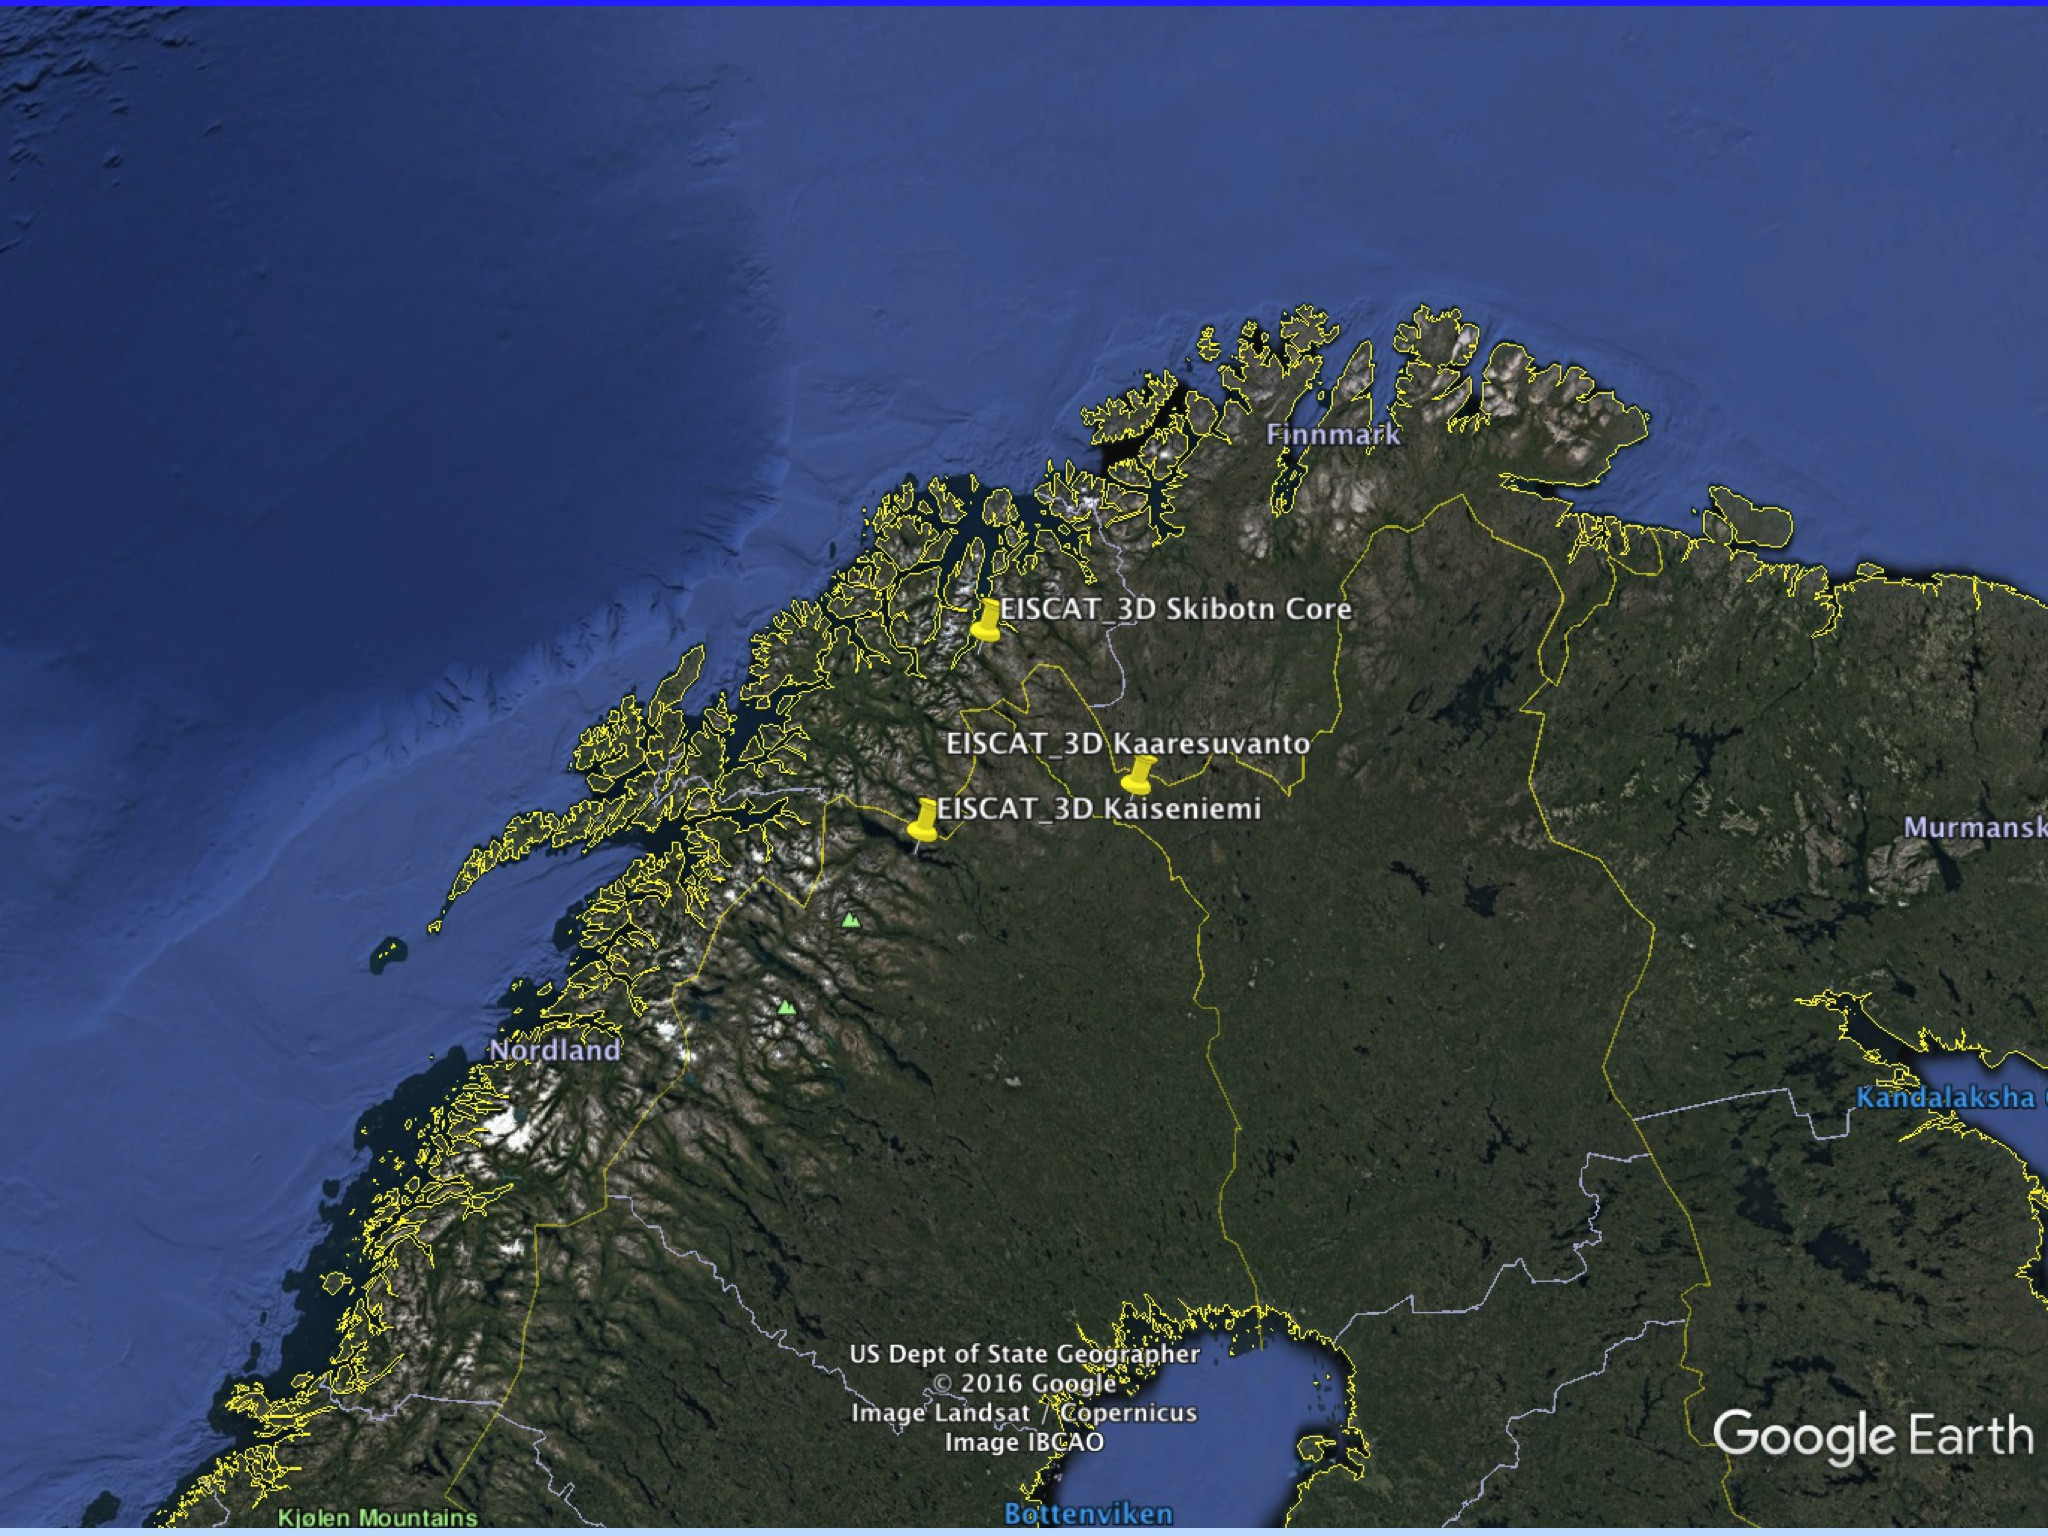
\includegraphics[height=2.7in]{EISCAT_3D_locations.jpg}
% \end{center}
% \vspace{-0.60in}
\vfill
% \note{\bitm 
    {\colblack Phase 1: One core station, two remote receiver sites.\\Remote control and data access}
    {\small \url{https://www.eiscat.se/about/eiscat3d7/}}
% \vfill
\end{center}
%       \item dimensions... 6m/80m dia.
%        \item TX 10 MW, high/low power modes, 
%        \item 60 degrees zenith angle, 
%        \item micro-second direction in point/look
%        \item white rabbit on-site
%        \item GPS between sites
%        \item explain time/volume integration for 3d operations
%       \eitm}
\end{frame}
